% !TeX program = xelatex
\documentclass[a4paper,10pt]{article}

% ============================================================================
% សន្លឹកកិច្ចការសិស្សបំពេញចន្លោះ ស-ខ្មៅ និងប្លង់ក្ដារខៀន/ចម្លើយគ្រូ (គ្មាន LCD / គ្មានកន្ត្រៃ)
% មេរៀនទី១ (៧.)៖ ការបង្គត់ចំនួនគត់ និងការប៉ាន់ស្មាន — ត្រូវគ្នា ១០០% នឹង LS_Plan_WN16.tex
% ============================================================================
\usepackage[a4paper, left=1.0cm, right=1.0cm, top=0.75cm, bottom=1.00cm, footskip=0.52cm]{geometry}
\usepackage{amsmath}
\usepackage{unicode-math}
\usepackage{fontspec}
\usepackage{array, colortbl}
\usepackage[table]{xcolor}
\usepackage{enumitem}
\usepackage{pifont}
\usepackage{fancyhdr}
\usepackage{lastpage}
\usepackage{tikz}
\usepackage[most]{tcolorbox}
\usetikzlibrary{calc, arrows.meta, decorations.pathreplacing, positioning, babel}

\makeatletter
\let\@expl@@@mark@update@singlecol@structures@@\relax
\makeatother

\providecommand{\NGSFindFonts}{%
  \IfFileExists{C:/Windows/Fonts/cambria.ttc}{%
    \def\NGSSysPath{C:/Windows/Fonts/}%
    \def\NGSUserPath{C:/Users/KIT/AppData/Local/Microsoft/Windows/Fonts/}%
  }{%
    \IfFileExists{./fonts/KhmerOSsiemreap.ttf}{\def\NGSSysPath{./fonts/}\def\NGSUserPath{./fonts/}}{%
    \IfFileExists{../fonts/KhmerOSsiemreap.ttf}{\def\NGSSysPath{../fonts/}\def\NGSUserPath{../fonts/}}{%
    \IfFileExists{../../fonts/KhmerOSsiemreap.ttf}{\def\NGSSysPath{../../fonts/}\def\NGSUserPath{../../fonts/}}{%
    \IfFileExists{../../../fonts/KhmerOSsiemreap.ttf}{\def\NGSSysPath{../../../fonts/}\def\NGSUserPath{../../../fonts/}}{%
    \IfFileExists{../../../../fonts/KhmerOSsiemreap.ttf}{\def\NGSSysPath{../../../../fonts/}\def\NGSUserPath{../../../../fonts/}}{%
    \IfFileExists{../../../../../fonts/KhmerOSsiemreap.ttf}{\def\NGSSysPath{../../../../../fonts/}\def\NGSUserPath{../../../../../fonts/}}{%
    \IfFileExists{../../../../../../fonts/KhmerOSsiemreap.ttf}{\def\NGSSysPath{../../../../../../fonts/}\def\NGSUserPath{../../../../../../fonts/}}{%
      \def\NGSSysPath{../../../../../../../fonts/}\def\NGSUserPath{../../../../../../../fonts/}%
    }}}}}}}%
  }%
}
\NGSFindFonts

\setmathfont[Path={\NGSSysPath}, FontIndex=1, Scale=1.02]{cambria.ttc}
\defaultfontfeatures{Ligatures=TeX}

\setmainfont[
  Path={\NGSUserPath}, Extension=.ttf, Script=Khmer,
  BoldFont={KhmerOSsiemreap}, BoldFeatures={FakeBold=1.8},
  ItalicFont={KhmerOSsiemreap}, ItalicFeatures={FakeSlant=0.25},
  BoldItalicFont={KhmerOSsiemreap}, BoldItalicFeatures={FakeBold=1.8, FakeSlant=0.25}
]{KhmerOSsiemreap}

\newfontfamily\muol[Path={\NGSUserPath}, Extension=.ttf, Script=Khmer]{KhmerOSmuollight}
\newfontfamily\TimesEn[Path={\NGSSysPath}, Extension=.ttf, BoldFont={timesbd}, ItalicFont={timesi}, BoldItalicFont={timesbi}]{times}
\newfontfamily\CalibriFont[Path={\NGSSysPath}, Extension=.ttf]{calibri}

\XeTeXlinebreaklocale "km"
\XeTeXlinebreakskip = 0pt plus 1pt minus 0.1pt

\definecolor{panelgray}{gray}{0.94}
\definecolor{headgray}{gray}{0.85}

\pagestyle{fancy}
\fancyhf{}
\renewcommand{\headrulewidth}{0pt}
\fancyfoot[L]{\fontsize{7.4pt}{9.5pt}\selectfont អនុវិទ្យាល័យព្រះក្រសាំង \en{|} គ្រូ៖ ហុក ប៊ុនថែន \en{|} មេរៀនទី១ (៧.) ការបង្គត់និងការប៉ាន់ស្មាន \en{|} ថ្ងៃអង្គារ ទី១០ ខែវិច្ឆិកា ឆ្នាំ២០២៦}
\fancyfoot[R]{\fontsize{7.8pt}{10pt}\selectfont ទំព័រ \en{\thepage\ / \pageref{LastPage}}}

\setlength{\parindent}{0pt}
\setlength{\parskip}{0pt}
\setlength{\tabcolsep}{4pt}
\newcolumntype{L}[1]{>{\raggedright\arraybackslash}p{#1}}
\newcolumntype{C}[1]{>{\centering\arraybackslash}p{#1}}

\newcommand{\en}[1]{{\TimesEn #1}}
\newcommand{\enbf}[1]{{\TimesEn\bfseries #1}}
\newcommand{\unit}[1]{\,\text{\en{#1}}}
\newcommand{\cnum}[1]{\mbox{\fontsize{10pt}{12pt}\selectfont\ding{\numexpr181+#1\relax}}}
\newcommand{\chkbox}{\tikz[baseline=-0.15ex]\draw[black, line width=0.85pt, fill=white] (0,0) rectangle (0.24cm,0.24cm);}
\newcommand{\ansbox}[1][1.75cm]{\,\tikz[baseline=-0.65ex]\draw[black, line width=0.65pt, fill=white] (0,0) rectangle (#1, 0.42cm);\,}
\newcommand{\dotline}[1][2.2cm]{\makebox[#1]{\dotfill}}

\newcommand{\pagebanner}[2]{%
  \begin{tcolorbox}[
    enhanced, sharp corners, colback=headgray, colframe=black,
    boxrule=1.05pt, boxsep=1pt, top=2.5pt, bottom=2.5pt, left=6pt, right=6pt,
    after skip=3.5pt
  ]
    {\muol\fontsize{9.0pt}{13.2pt}\selectfont #1}\hfill{\fontsize{8.0pt}{11.2pt}\selectfont\textbf{#2}}
  \end{tcolorbox}%
}

\newcommand{\secstrip}[2]{%
  \vspace{3pt}%
  \begin{tcolorbox}[
    enhanced, sharp corners, colback=panelgray, colframe=black,
    boxrule=0.8pt, boxsep=0.8pt, top=2pt, bottom=2pt, left=5pt, right=5pt,
    after skip=3pt
  ]
    {\muol\fontsize{8.5pt}{12.2pt}\selectfont #1}\hfill{\fontsize{7.8pt}{10.8pt}\selectfont\textit{#2}}
  \end{tcolorbox}%
}

\begin{document}
\fontsize{9.5pt}{14.5pt}\selectfont

% ============================================================================
% ទំព័រទី ១៖ សន្លឹកកិច្ចការសិស្ស (ផ្នែកមុខ៖ E1 -> E2 -> E3)
% ============================================================================
\pagebanner{សន្លឹកកិច្ចការសិស្ស \enbf{(}៧\enbf{.} ការបង្គត់ចំនួនគត់ និងការប៉ាន់ស្មាន\enbf{)} \enbf{--} ផ្នែកមុខ}{ថ្នាក់ទី៧ \en{|} សៀវភៅគោល ទំ.១០--១១}

\begin{tcolorbox}[
  enhanced, sharp corners, colback=white, colframe=black,
  boxrule=0.8pt, boxsep=1.5pt, top=3.5pt, bottom=3.5pt, left=5pt, right=5pt,
  after skip=4pt
]
  \fontsize{9.0pt}{13.0pt}\selectfont
  \textbf{ឈ្មោះសិស្ស៖} \dotline[4.3cm] \quad
  \textbf{សមាជិកក្រុម៖} \dotline[4.3cm] \quad
  \textbf{ថ្នាក់ទី៖} ៧\dotline[0.9cm] \quad
  \textbf{ក្រុមទី៖} \dotline[1.0cm]
\end{tcolorbox}

% --- E1 Engage ---
\secstrip{ផ្នែកទី ១ \enbf{(E1 - Engage)} ៖ បេសកកម្មអន្ទាក់ការបង្គត់ $15\,824$ ត្រឹមខ្ទង់ពាន់}{រយៈពេល ៣ នាទី (គូស \ding{51} ក្នុង \chkbox)}

\begin{tcolorbox}[
  enhanced, sharp corners, colback=white, colframe=black,
  boxrule=0.8pt, boxsep=2pt, top=4pt, bottom=4pt, left=6pt, right=6pt
]
  គេចង់បង្គត់ចំនួន $15\,824$ យកត្រឹម\textbf{ខ្ទង់ពាន់} (ឧទាហរណ៍ ២ ទំ.១១)៖\\[3pt]
  $\bullet$ \textbf{តើសិស្សរូបណាបង្គត់បានត្រឹមត្រូវ?} \quad
  \chkbox\ \textbf{សិស្ស ក៖} $15\,000$ (មើលលេខ $2 < 5$) \quad
  \chkbox\ \textbf{សិស្ស ខ៖} $16\,000$ (មើលលេខ $8 > 5$)\\[3pt]
  $\bullet$ \textbf{ហេតុផល៖} លេខនៅខាងស្ដាំជាប់ខ្ទង់ពាន់ ($5$) គឺលេខ \dotline[1.1cm] ដែលធ្វើឱ្យ $15\,824$ នៅជិត \dotline[1.8cm] ជាង ។
\end{tcolorbox}

\vfill

% --- E2 Explore ---
\secstrip{ផ្នែកទី ២ \enbf{(E2 - Explore)} ៖ បន្ទាត់ចំនួនចំណុចកណ្ដាល និងការប៉ាន់ស្មានផលបូក (ទំ.១០--១១)}{រយៈពេល ១១ នាទី}

\textbf{សកម្មភាព ១ (\en{E2-A} — ៥ នាទី)៖ ការបង្គត់លើបន្ទាត់ចំនួនធៀបចំណុចកណ្ដាល (ឧទាហរណ៍ ១ ក, ខ ទំ.១០)}

\begin{tcolorbox}[
  enhanced, sharp corners, colback=white, colframe=black,
  boxrule=0.8pt, boxsep=2.5pt, top=4pt, bottom=4pt, left=6pt, right=6pt
]
  \begin{minipage}{8.9cm}
    \textbf{ក.} បង្គត់ $647$ ត្រឹមខ្ទង់ដប់ (ចំណុចកណ្ដាល $645$)៖\\[2pt]
    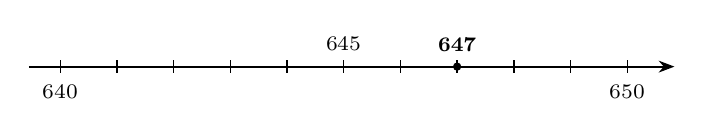
\begin{tikzpicture}[x=1cm, y=1cm, every node/.style={font=\fontsize{7.5pt}{9.5pt}\selectfont, text=black}]
      \draw[-{Stealth[length=2mm]}, black, line width=0.8pt] (0,0) -- (8.2,0);
      \foreach \x in {0.4, 1.12, 1.84, 2.56, 3.28, 4.0, 4.72, 5.44, 6.16, 6.88, 7.6}
        \draw[black, line width=0.5pt] (\x,-0.08) -- (\x,0.08);
      \node[below=3pt] at (0.4,0) {$640$};
      \node[above=2pt] at (4.0,0) {$645$};
      \fill[black] (5.44,0) circle (1.5pt) node[above=2pt] {$\mathbf{647}$};
      \node[below=3pt] at (7.6,0) {$650$};
    \end{tikzpicture}\\[2pt]
    ដូចនេះ $647 \approx$ \ansbox[1.6cm] (បង្គត់\dotline[1.3cm])
  \end{minipage}\hfill
  \begin{minipage}{8.9cm}
    \textbf{ខ.} បង្គត់ $2\,931$ ត្រឹមខ្ទង់រយ (ចំណុចកណ្ដាល $2\,950$)៖\\[2pt]
    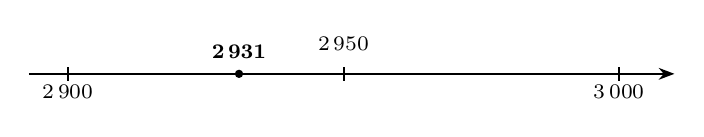
\begin{tikzpicture}[x=1cm, y=1cm, every node/.style={font=\fontsize{7.5pt}{9.5pt}\selectfont, text=black}]
      \draw[-{Stealth[length=2mm]}, black, line width=0.8pt] (0,0) -- (8.2,0);
      \draw[black, line width=0.65pt] (0.5,-0.09) -- (0.5,0.09) node[below=3pt] {$2\,900$};
      \fill[black] (2.67,0) circle (1.5pt) node[above=2pt] {$\mathbf{2\,931}$};
      \draw[black, line width=0.65pt] (4.0,-0.09) -- (4.0,0.09) node[above=2pt] {$2\,950$};
      \draw[black, line width=0.65pt] (7.5,-0.09) -- (7.5,0.09) node[below=3pt] {$3\,000$};
    \end{tikzpicture}\\[2pt]
    ដូចនេះ $2\,931 \approx$ \ansbox[1.7cm] (បង្គត់\dotline[1.3cm])
  \end{minipage}
\end{tcolorbox}

\vspace{4pt}
\textbf{សកម្មភាព ២ (\en{E2-B} — ៦ នាទី)៖ ការពិនិត្យខ្ទង់ខាងស្ដាំ និងការប៉ាន់ស្មានផលបូក (ឧទាហរណ៍ ទំ.១១)}

\begin{tcolorbox}[
  enhanced, sharp corners, colback=white, colframe=black,
  boxrule=0.8pt, boxsep=2.5pt, top=4.5pt, bottom=4.5pt, left=6pt, right=6pt
]
  $\bullet$ \textbf{ឧទាហរណ៍ ២៖} បង្គត់ $15\,824$៖ ១) ត្រឹមខ្ទង់រយ (មើលលេខ $2$) $\approx$ \dotline[1.8cm] $\mid$ ២) ត្រឹមខ្ទង់ពាន់ (មើលលេខ $8$) $\approx$ \ansbox[1.8cm]\\[3.5pt]
  $\bullet$ \textbf{ការប៉ាន់ស្មានផលបូក (ទំ.១១)៖} $732 + 576 + 342 \approx$ \dotline[1.3cm] $+$ \dotline[1.3cm] $+$ \dotline[1.3cm] $=$ \ansbox[1.8cm]
\end{tcolorbox}

\vfill

% --- E3 Explain ---
\secstrip{ផ្នែកទី ៣ \enbf{(E3 - Explain)} ៖ វិធានជាទូទៅ និងធនាគារហេតុផល \enbf{B\&W}}{រយៈពេល ៦ នាទី}

\begin{tcolorbox}[
  enhanced, sharp corners, colback=white, colframe=black,
  boxrule=0.85pt, boxsep=2.5pt, top=4pt, bottom=4pt, left=6pt, right=6pt
]
  ក្នុងការបង្គត់ចំនួន គេត្រូវមើលតែលេខ\textbf{មួយខ្ទង់នៅខាងស្ដាំបន្ទាប់}ពីខ្ទង់ដែលចង់បង្គត់៖\\[3pt]
  ១) បើមានតម្លៃពី $0$ ដល់ \dotline[0.9cm] ត្រូវ\textbf{បង្គត់ចុះ} (រក្សាខ្ទង់គោលដៅ ជំនួសគ្រប់ខ្ទង់ខាងស្ដាំដោយលេខ $0$) ។\\[3pt]
  ២) បើមានតម្លៃពី \dotline[0.9cm] ដល់ $9$ ត្រូវ\textbf{បង្គត់ឡើង} (បន្ថែម $+1$ ទៅលើខ្ទង់គោលដៅ ជំនួសគ្រប់ខ្ទង់ខាងស្ដាំដោយលេខ $0$) ។\\[4pt]
  \tikz\draw[black, dashed, line width=0.5pt] (0,0) -- (18.4cm,0);\\[3.5pt]
  \fontsize{8.8pt}{13.0pt}\selectfont
  \textbf{ធនាគារហេតុផល (\en{Warrant Bank})៖} \quad
  \cnum{1} \textbf{បង្គត់ចុះ ($0\text{--}4$)៖} រក្សាខ្ទង់គោលដៅ ដាក់ $0$ ខាងស្ដាំ \quad
  \cnum{2} \textbf{បង្គត់ឡើង ($5\text{--}9$)៖} បូក $+1$ លើខ្ទង់គោលដៅ\\
  \cnum{3} \textbf{ប៉ាន់ស្មានរហ័ស៖} បង្គត់តួនីមួយៗជាមុនសិន រួចទើបគណនា ($\approx$) \quad
  \cnum{4} \textbf{ត្រាទុក $9+1=10$៖} បន្ត $+1$ ទៅខ្ទង់ខាងឆ្វេងបន្ទាប់
\end{tcolorbox}

% ============================================================================
% ទំព័រទី ២៖ សន្លឹកកិច្ចការសិស្ស (ផ្នែកខាងខ្នង៖ E4 -> E5 -> កិច្ចការផ្ទះ)
% ============================================================================
\clearpage
\pagebanner{សន្លឹកកិច្ចការសិស្ស \enbf{(}៧\enbf{.} ការបង្គត់ចំនួនគត់ និងការប៉ាន់ស្មាន\enbf{)} \enbf{--} ផ្នែកខាងខ្នង}{ថ្នាក់ទី៧ \en{|} សៀវភៅគោល ទំ.១១ និង ទំ.១៤}

% --- E4 Elaborate ---
\secstrip{ផ្នែកទី ៤ \enbf{(E4 - Elaborate)} ៖ លំហាត់គំរូ — ការប៉ាន់ស្មានចម្លើយប្រមាណវិធី (ទំ.១១)}{រយៈពេល ១០ នាទី}

\begin{tcolorbox}[
  enhanced, sharp corners, colback=white, colframe=black,
  boxrule=0.8pt, boxsep=2.5pt, top=4.5pt, bottom=4.5pt, left=6pt, right=6pt
]
  \textbf{លំហាត់គំរូ (ទំ.១១)៖} ធ្វើការប៉ាន់ស្មានចម្លើយនៃប្រមាណវិធី $870 \times 38 \div 95$ ។\\[3.5pt]
  $\bullet$ \textbf{ជំហានទី១ (បង្គត់តួនីមួយៗឱ្យងាយគណនា)៖} $870 \approx$ \dotline[1.4cm], \quad $38 \approx$ \dotline[1.2cm], \quad $95 \approx$ \dotline[1.4cm]\\[3.5pt]
  $\bullet$ \textbf{ជំហានទី២ (គណនាក្នុងចិត្ត — \cnum{3})៖} $870 \times 38 \div 95 \approx$ \dotline[1.4cm] $\times 40 \div 100 =$ \dotline[1.8cm] $\div 100 =$ \ansbox[1.8cm]\\[3.5pt]
  \fontsize{8.8pt}{12.8pt}\selectfont
  \textbf{ឆ្លុះបញ្ចាំង (\en{EIA Looking-Back})៖} បើសិស្សម្នាក់គណនាច្រឡំខ្ទង់ឃើញ $3\,480$ តើសមហេតុផលធៀបនឹង $360$ ដែរឬទេ? \dotline[2.4cm]
\end{tcolorbox}

\vfill

% --- E5 Evaluate ---
\secstrip{ផ្នែកទី ៥ \enbf{(E5 - Evaluate)} ៖ លំហាត់ប្រតិបត្តិ (ទំ.១១) សំណួរវិនិច្ឆ័យ \enbf{A--D} និងសំបុត្រចេញ}{រយៈពេល ១០ នាទី}

\begin{tcolorbox}[
  enhanced, sharp corners, colback=white, colframe=black,
  boxrule=0.8pt, boxsep=2.5pt, top=4.5pt, bottom=4.5pt, left=6pt, right=6pt
]
  \textbf{១) ប្រតិបត្តិជាក្រុមតូច ៣ នាក់ (សៀវភៅគោល ទំ.១១)៖} បង្គត់ចំនួនខាងក្រោមយកត្រឹមខ្ទង់ដប់ ខ្ទង់រយ និងខ្ទង់ពាន់៖\\[3.5pt]
  {\renewcommand{\arraystretch}{1.28}
  \begin{tabular}{|L{4.1cm}|C{4.3cm}|C{4.3cm}|C{4.3cm}|}
    \hline
    \cellcolor{headgray}\textbf{ចំនួនដើម (ទំ.១១)} &
    \cellcolor{headgray}\textbf{បង្គត់ត្រឹមខ្ទង់ដប់} &
    \cellcolor{headgray}\textbf{បង្គត់ត្រឹមខ្ទង់រយ} &
    \cellcolor{headgray}\textbf{បង្គត់ត្រឹមខ្ទង់ពាន់} \\[2pt] \hline
    ក. $7\,663\,692$ & \dotline[3.4cm] & \dotline[3.4cm] & \dotline[3.4cm] \\ \hline
    ខ. $996\,972$ (\emph{ប្រយ័ត្ន \cnum{4}}) & \dotline[3.4cm] & \dotline[3.4cm] & \dotline[3.4cm] \\ \hline
    គ. $3\,500\,004$ & \dotline[3.4cm] & \dotline[3.4cm] & \dotline[3.4cm] \\ \hline
  \end{tabular}}\\[4pt]
  \textbf{២) បិទបេសកកម្ម \en{E1}៖} សិស្ស \dotline[1.0cm] ត្រឹមត្រូវ ព្រោះ $15\,824 \approx$ \dotline[1.8cm] (ខ្ទង់រយគឺ $8 \ge 5$ — \cnum{2}) ។
\end{tcolorbox}

\vspace{4pt}

\begin{tcolorbox}[
  enhanced, sharp corners, colback=white, colframe=black,
  boxrule=0.8pt, boxsep=2.5pt, top=4.5pt, bottom=4.5pt, left=6pt, right=6pt
]
  \textbf{៣) សំណួរវិនិច្ឆ័យ \en{A--D} (បង្គត់ចំនួន $49\,962$ យកត្រឹមខ្ទង់រយ — គូសរង្វង់ រួចលើកម្រាមដៃ ១--៤)៖}\\[3.5pt]
  \textbf{\en{A.}} $49\,900$ \qquad\qquad
  \textbf{\en{B.}} $49\,000$ \qquad\qquad
  \textbf{\en{C.}} $50\,000$ \qquad\qquad
  \textbf{\en{D.}} $5\,000$\\[4.5pt]
  \tikz\draw[black, dashed, line width=0.5pt] (0,0) -- (18.4cm,0);\\[3.5pt]
  \textbf{៤) សំបុត្រចេញ ៦០ វិនាទី៖} ប៉ាន់ស្មានផលគុណ $592 \times 41 \approx$ \dotline[1.4cm] $\times$ \dotline[1.2cm] $=$ \ansbox[2.0cm] ។
\end{tcolorbox}

\vfill

% --- Homework ---
\begin{tcolorbox}[
  enhanced, sharp corners, colback=panelgray, colframe=black,
  boxrule=0.95pt, boxsep=2.5pt, top=4pt, bottom=4pt, left=6pt, right=6pt
]
  {\muol\fontsize{9.0pt}{13.0pt}\selectfont កិច្ចការផ្ទះ \enbf{(}សៀវភៅគោល ទំ.១៤ លេខ ៦ និង លេខ ៧\enbf{)}}\\[3pt]
  \fontsize{8.8pt}{12.8pt}\selectfont
  $\bullet$ \textbf{លេខ ៦ (បង្គត់យកត្រឹមខ្ទង់ដប់ ខ្ទង់រយ និងខ្ទង់ពាន់)៖} \quad ក. $149\,905$ \quad ខ. $384\,000$ \quad គ. $2\,990\,346$ \quad ឃ. $6\,754\,550$ ។\\[2pt]
  $\bullet$ \textbf{លេខ ៧ (ធ្វើការប៉ាន់ស្មានតម្លៃ)៖} \quad ក. $398 + 527$ \qquad ខ. $3\,648 \times 999$ \qquad គ. $4\,201 \div 58$ ។
\end{tcolorbox}

% ============================================================================
% ទំព័រទី ៣៖ ទំព័រគ្រូបង្រៀន (គំរូប្លង់ក្ដារខៀន ៣ ផ្នែក + ចម្លើយផ្ទៀងផ្ទាត់រហ័ស)
% ============================================================================
\clearpage
\pagebanner{ទំព័រគ្រូបង្រៀន ៖ ប្លង់ក្ដារខៀន \enbf{(}គ្មាន \enbf{LCD)} និងចម្លើយផ្ទៀងផ្ទាត់រហ័ស}{៧. ការបង្គត់ចំនួនគត់ និងការប៉ាន់ស្មាន (\en{WN16})}

\secstrip{១. គំរូប្លង់បែងចែកក្ដារខៀន ៣ ផ្នែក សម្រាប់ថ្នាក់រៀនគ្មាន \enbf{LCD}}{សម្រាប់គ្រូប្រើដីស/ហ្វឺត}

\begin{center}
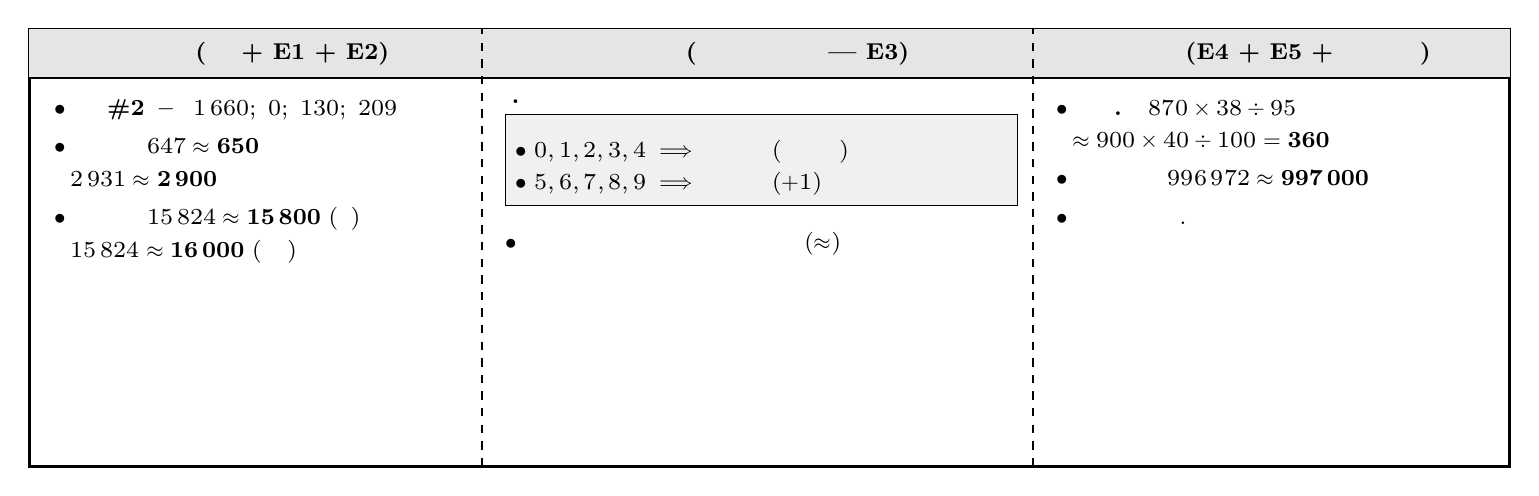
\begin{tikzpicture}[x=1cm, y=1cm, every node/.style={font=\fontsize{8.3pt}{11.8pt}\selectfont, text=black}]
  \draw[black, line width=1.1pt] (0,0) rectangle (18.8,5.55);
  \fill[gray!20] (0,4.93) rectangle (18.8,5.55);
  \draw[black, line width=0.7pt] (0,4.93) -- (18.8,4.93);
  \draw[black, dashed, line width=0.7pt] (5.75,0) -- (5.75,5.55);
  \draw[black, dashed, line width=0.7pt] (12.75,0) -- (12.75,5.55);

  \node at (2.875,5.24) {\textbf{ផ្នែកឆ្វេង (កំណែ + \en{E1} + \en{E2})}};
  \node at (9.25,5.24) {\textbf{ផ្នែកកណ្ដាល (ខ្លឹមសារគោលរក្សាទុក — \en{E3})}};
  \node at (15.775,5.24) {\textbf{ផ្នែកស្ដាំ (\en{E4} + \en{E5} + កិច្ចការផ្ទះ)}};

  % Left
  \node[anchor=north west, text width=5.30cm] at (0.20,4.78) {%
    $\bullet$ \textbf{កំណែ \#2 ខ–ង៖} $1\,660;\ 0;\ 130;\ 209$\\[2pt]
    $\bullet$ \textbf{ឧទាហរណ៍ ១៖} $647 \approx \mathbf{650}$\\
    \hspace*{0.2cm}$2\,931 \approx \mathbf{2\,900}$\\[2pt]
    $\bullet$ \textbf{ឧទាហរណ៍ ២៖} $15\,824 \approx \mathbf{15\,800}$ (រយ)\\
    \hspace*{0.2cm}$15\,824 \approx \mathbf{16\,000}$ (ពាន់)
  };

  % Center
  \node[anchor=north west, text width=6.65cm] at (5.92,4.78) {%
    {\muol\fontsize{8.4pt}{12pt}\selectfont ៧\enbf{.} ការបង្គត់ចំនួនគត់ និងការប៉ាន់ស្មាន}\\[3pt]
    \tikz\node[draw=black, fill=gray!12, inner sep=3.5pt, text width=6.25cm]{%
      មើលលេខ\textbf{មួយខ្ទង់នៅខាងស្ដាំជាប់}៖\\
      $\bullet$ $0, 1, 2, 3, 4 \implies$ បង្គត់ចុះ (រក្សាដដែល)\\
      $\bullet$ $5, 6, 7, 8, 9 \implies$ បង្គត់ឡើង ($+1$)
    };\\[4pt]
    $\bullet$ \textbf{ការប៉ាន់ស្មាន៖} បង្គត់តួនីមួយៗជាមុន រួចគណនា ($\approx$)
  };

  % Right
  \node[anchor=north west, text width=5.65cm] at (12.92,4.78) {%
    $\bullet$ \textbf{គំរូទំ.១១៖} $870\times 38\div 95$\\
    \hspace*{0.2cm}$\approx 900\times 40\div 100 = \mathbf{360}$\\[2pt]
    $\bullet$ \textbf{ប្រតិបត្តិ ខ៖} $996\,972 \approx \mathbf{997\,000}$\\[2pt]
    $\bullet$ \textbf{កិច្ចការផ្ទះ៖} ទំ.១៤ លេខ ៦ និង លេខ ៧
  };
\end{tikzpicture}
\end{center}

\vfill
\secstrip{២. ចម្លើយផ្ទៀងផ្ទាត់រហ័សសម្រាប់សន្លឹកកិច្ចការសិស្ស \enbf{(}ទំព័រ ១ និង ទំព័រ ២\enbf{)}}{\en{Answer Key}}

\begin{tcolorbox}[
  enhanced, sharp corners, colback=white, colframe=black,
  boxrule=0.8pt, boxsep=2.5pt, top=4.5pt, bottom=4.5pt, left=6pt, right=6pt
]
  \fontsize{8.9pt}{13.2pt}\selectfont
  $\bullet$ \textbf{ផ្នែក \en{E1}៖} \textbf{សិស្ស ខ} ត្រឹមត្រូវ ($16\,000$) ព្រោះខ្ទង់រយនៅខាងស្ដាំជាប់ខ្ទង់ពាន់គឺលេខ $8$ ($\ge 5$) ។\\[2pt]
  $\bullet$ \textbf{ផ្នែក \en{E2}៖} \textbf{សកម្មភាព ១៖} ក. $647 \approx \mathbf{650}$ (ឡើង); ខ. $2\,931 \approx \mathbf{2\,900}$ (ចុះ) ។ \textbf{សកម្មភាព ២៖} $15\,800$ និង $16\,000$; $700+600+300 = \mathbf{1\,600}$ ។\\[2pt]
  $\bullet$ \textbf{ផ្នែក \en{E4}៖} $900 \times 40 \div 100 = 36\,000 \div 100 = \mathbf{360}$ ។ \en{EIA}៖ មិនសមហេតុផលទេ (ខុសខ្ទង់ដល់ $10$ ដង) ។\\[2pt]
  $\bullet$ \textbf{ផ្នែក \en{E5}៖} \textbf{១) ប្រតិបត្តិទំ.១១៖} ក. $7\,663\,690;\ 7\,663\,700;\ 7\,664\,000$ $\mid$ ខ. $996\,970;\ 997\,000;\ 997\,000$ $\mid$ គ. $3\,500\,000$ (ទាំងបី) ។ \textbf{២) បិទ \en{E1}៖} សិស្ស ខ ($16\,000$) ។ \textbf{៣) វិនិច្ឆ័យ \en{A--D}៖} \textbf{ជម្រើស \en{C}} ($50\,000$) ។ \textbf{៤) សំបុត្រចេញ៖} $600\times 40 = \mathbf{24\,000}$ ។
\end{tcolorbox}

\vfill
\secstrip{៣. ចម្លើយលម្អិតនៃកិច្ចការផ្ទះ \enbf{(}សៀវភៅគោល ទំ.១៤ លេខ ៦ និង លេខ ៧\enbf{)}}{សៀវភៅគោល ទំ.១៤}

\begin{tcolorbox}[
  enhanced, sharp corners, colback=white, colframe=black,
  boxrule=0.8pt, boxsep=2.5pt, top=4.5pt, bottom=4.5pt, left=6pt, right=6pt
]
  \fontsize{8.7pt}{12.8pt}\selectfont
  $\bullet$ \textbf{លេខ ៦ (ដប់; រយ; ពាន់)៖} ក. $149\,910;\ 149\,900;\ 150\,000$ $\mid$ ខ. $384\,000$ (ទាំងបី) $\mid$ គ. $2\,990\,350;\ 2\,990\,300;\ 2\,990\,000$ $\mid$ ឃ. $6\,754\,550;\ 6\,754\,600;\ 6\,755\,000$ ។\\[2pt]
  $\bullet$ \textbf{លេខ ៧ (ប៉ាន់ស្មាន)៖} ក. $398+527 \approx 400+500 = \mathbf{900}$ (ឬ $400+530=\mathbf{930}$) $\mid$ ខ. $3\,648\times 999 \approx 3\,600\times 1\,000 = \mathbf{3\,600\,000}$ (ឬ $3\,650\times 1\,000 = \mathbf{3\,650\,000}$) $\mid$ គ. $4\,201\div 58 \approx 4\,200\div 60 = \mathbf{70}$ ។
\end{tcolorbox}

\vfill
\secstrip{៤. ចំណុចប្រុងប្រយ័ត្នគរុកោសល្យសម្រាប់គ្រូ \enbf{(}ការយល់ច្រឡំ និងកំហុសពុម្ពទំ.១១\enbf{)}}{\en{Pedagogical Watchlist}}

\begin{tcolorbox}[
  enhanced, sharp corners, colback=panelgray, colframe=black,
  boxrule=0.85pt, boxsep=2.5pt, top=4.5pt, bottom=4.5pt, left=6pt, right=6pt
]
  \fontsize{8.6pt}{12.7pt}\selectfont
  $\bullet$ \textbf{កំហុសពុម្ពក្នុងសៀវភៅគោលទំ.១១ (២ កន្លែង)៖} ១) ក្នុងឧទាហរណ៍ ២ បោះពុម្ព «$15\,824 = 1\,6\,0\,0$» (បាត់សូន្យ ១ ខ្ទង់) ត្រូវកែជា $\mathbf{16\,000}$ និងប្រើសញ្ញា $\approx$; ២) ក្នុងឧទាហរណ៍ប៉ាន់ស្មានបោះពុម្ព «$16.000$» ត្រូវកែជា $\mathbf{1\,600}$ ។\\[2pt]
  $\bullet$ \textbf{អន្ទាក់បង្គត់ពីរដងបន្តគ្នា៖} ចំពោះ $149\,905$ (លេខ ៦ ក) ត្រឹមខ្ទង់រយត្រូវមើលខ្ទង់ដប់ ($0 < 5 \implies 149\,900$) ហាមបង្គត់ពី $149\,910$ បន្តទៅ $150\,000$!
\end{tcolorbox}

\end{document}
